\documentclass[12pt]{article}
\usepackage[english]{babel}
\usepackage[utf8x]{inputenc}
\usepackage{fullpage}
\usepackage{pythonhighlight}
\usepackage{graphicx}
\usepackage{geometry}
\usepackage{cite}
\usepackage{enumitem}
\usepackage{sectsty}
\usepackage{hyperref}

\usepackage{listings}
\usepackage{graphicx}
\usepackage{float}
\usepackage{subcaption}
\usepackage{mwe}
\usepackage{blindtext}
\usepackage{scrextend}
\addtokomafont{labelinglabel}{\sffamily}
\geometry{
	a4paper,
	top=0.89in,
	bottom=0.89in,
	left=0.9in,
	right=0.9in
}

\renewcommand{\thesubsection}{\thesection.\alph{subsection}}

% load package with some of the available options - you may not need this!
%\usepackage[framed,numbered,autolinebreaks,useliterate]{mcode}
\usepackage{titling}
\setlength{\droptitle}{-2cm}
\title{Programming Assignment 2 - Clustering}
\date{}
\author{\fontsize{12}{12}\selectfont Yang Ji\\ \fontsize{12}{12}\selectfont Student No. 56064832}
\sectionfont{\fontsize{12}{12}\selectfont}

\begin{document}
\maketitle
\section{\fontsize{16}{16}\selectfont Clustering synthetic data}
\subsection{Implementation}
Source code can be found at \url{https://github.com/yangji12138/machine-learning/tree/master/Programming2}

\vspace{1em}
\noindent\textbf{File Structure:}

\begin{labeling}{alligator}
\item [main.m] Main function to display the experiment results
\item [kmean.m] kmeans algorithm for \(1^{st}\) problem
\item [kmean2.m] kmeans algorithm for \(2^{nd}\) problem (different distance measurement)
\item [em\_gaussian.m] EM-GMM algorithm
\item [init\_para.m] Initialization of parameters in EM-GMM model
\item [calcP.m] Calculation of probability function in EM-GMM model
\item [meanshift.m] meanshift algorithm 
\item [plotf.m] Plot Clustering results
\end{labeling}

\subsection{Running algorithms on the three synthetic data}

\begin{figure}[H]
\minipage{0.30\textwidth}
  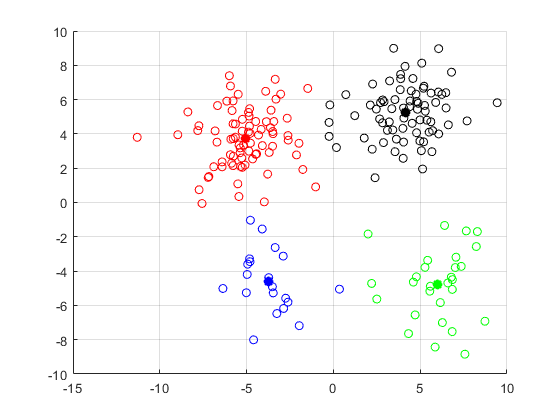
\includegraphics[width=\linewidth]{figs/1-b-kmeans-a.png}
  \caption{Data\_A}\label{fig:kmeans-a}
\endminipage\hfill
\minipage{0.30\textwidth}
  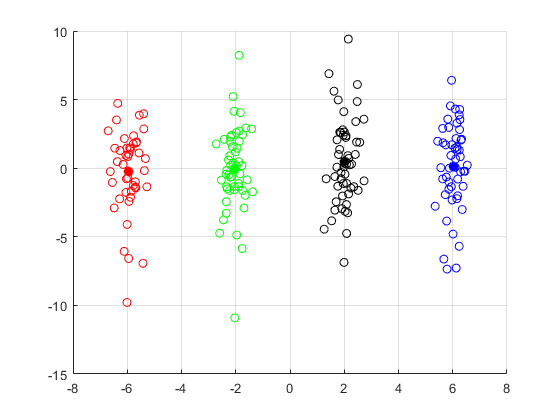
\includegraphics[width=\linewidth]{figs/1-b-kmeans-b.png}
  \caption{Data\_B}\label{fig:kmeans-b}
\endminipage\hfill
\minipage{0.30\textwidth}%
  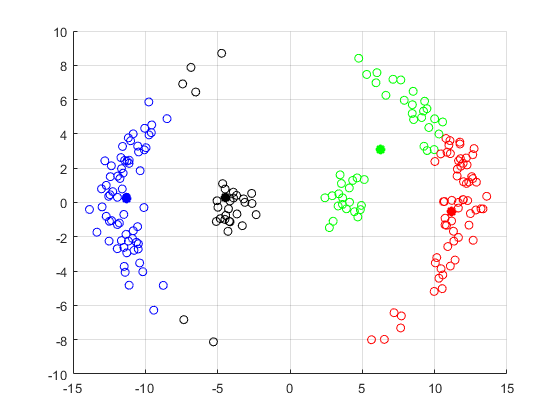
\includegraphics[width=\linewidth]{figs/1-b-kmeans-c.png}
  \caption{Data\_C}\label{fig:kmeans-c}
\endminipage
\caption{K-means Algorithm}
\end{figure}

\begin{figure}[H]
	\minipage{0.30\textwidth}
	  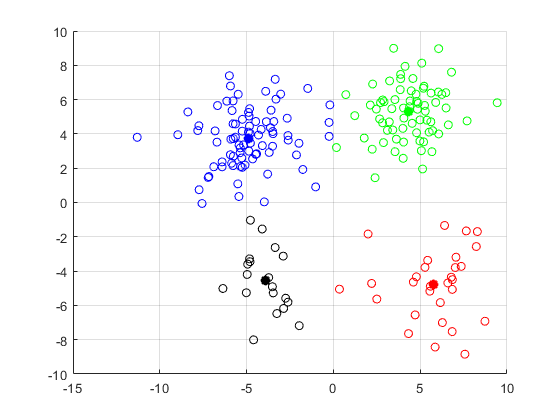
\includegraphics[width=\linewidth]{figs/1-b-em-a.png}
	  \caption{Data\_A}\label{fig:kmeans-a}
	\endminipage\hfill
	\minipage{0.30\textwidth}
	  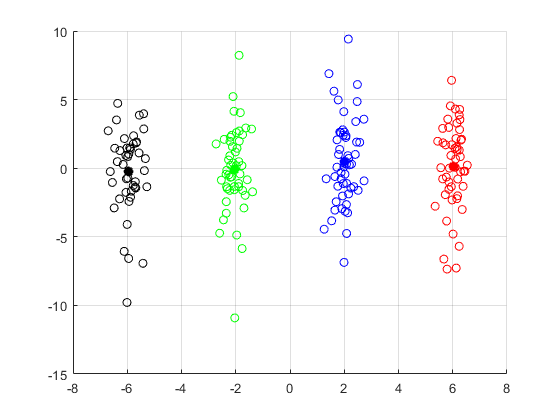
\includegraphics[width=\linewidth]{figs/1-b-em-b.png}
	  \caption{Data\_B}\label{fig:kmeans-b}
	\endminipage\hfill
	\minipage{0.30\textwidth}%
	  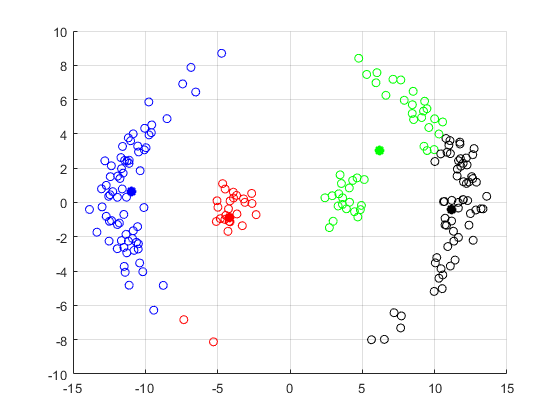
\includegraphics[width=\linewidth]{figs/1-b-em-c.png}
	  \caption{Data\_C}\label{fig:kmeans-c}
	\endminipage
	\caption{EM-GMM Algorithm}
\end{figure}

\begin{figure}[H]
	\minipage{0.30\textwidth}
	  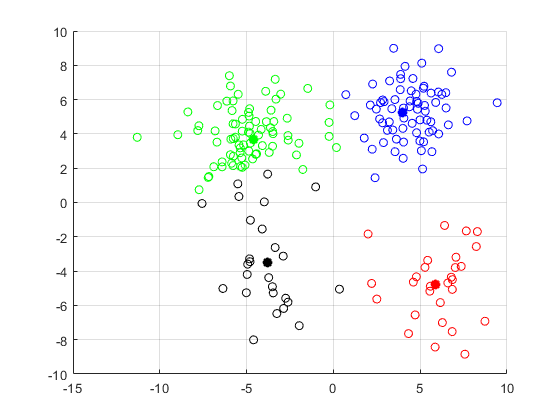
\includegraphics[width=\linewidth]{figs/1-b-meanshift-a.png}
	  \caption{Data\_A \\$h$ = 5}\label{fig:kmeans-a}
	\endminipage\hfill
	\minipage{0.30\textwidth}
	  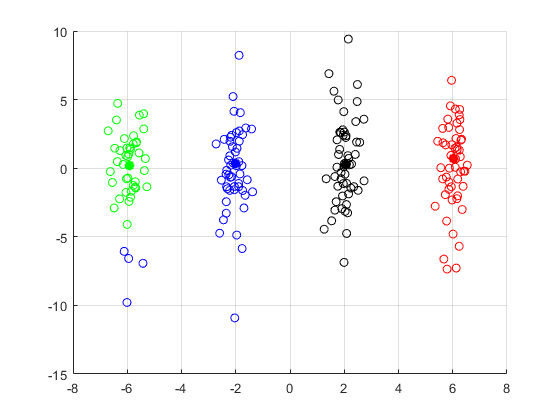
\includegraphics[width=\linewidth]{figs/1-b-meanshift-b.png}
	  \caption{Data\_B \\$h$ = 3}\label{fig:kmeans-b}
	\endminipage\hfill
	\minipage{0.30\textwidth}%
	  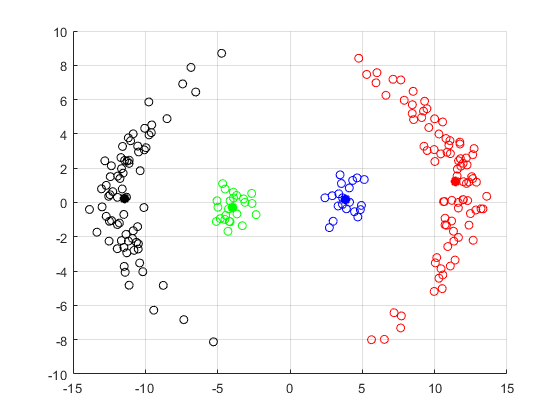
\includegraphics[width=\linewidth]{figs/1-b-meanshift-c.png}
	  \caption{Data\_C \\$h$ = 4}\label{fig:kmeans-c}
	\endminipage
	\caption{Mean-Shift Algorithm}
\end{figure}

\textbf{Conclusion:}\\

In the experiments, I using the given three algorithms (K-means, EM-GMM and Mean-Shift) to do the clustering tasks. More specifically, K-means and EM-GMM are parametric clustering and mean-shift is non-parametric clustering method. In each figure, I also utilize block spots to mark the center of each cluster. 

Observing the experiment results, I find that the performance of K-means and EM-GMM is similar. They both can correctly cluster the data points into four classes. And the center point of each cluster can truly reflect the character of each cluster. However, compared to the original figures, these two algorithms have some deviations. They fail to discriminate the last column in Data\_C. One reason is from different initial sets of data points. Different Initialization points can lead to totally different clustering results.

For non-parametric method (Mean-Shift), we can adjust the parameter (bandwidth h) to do the clustering. It is worth nothing that the black point in the Figure 12 is the local peak point instead of center point. We find that it works very well when we choose a appropriate parameter (bandwidth h). Although it get rid of the choice of parameter, it suffers from the adjustment on bandwidth h. The details will be shown as follows.

\subsection{Sensitivity of bandwidth h}

\begin{figure}[H]
    \centering % <-- added
\begin{subfigure}{0.25\textwidth}
  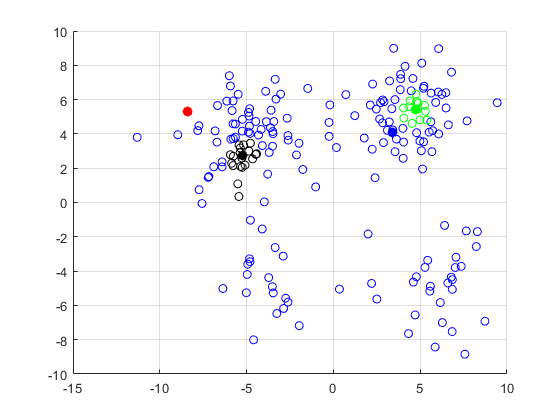
\includegraphics[width=\linewidth]{figs/1-b-meanshift-a-7.png}
  \caption{$h$ = 1}
  \label{fig:1}
\end{subfigure}\hfil % <-- added
\begin{subfigure}{0.25\textwidth}
  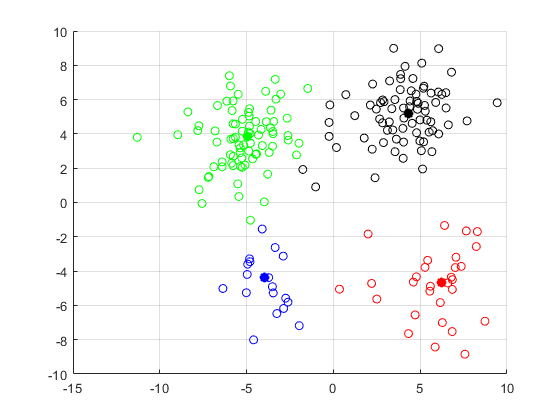
\includegraphics[width=\linewidth]{figs/1-b-meanshift-a-3.png}
  \caption{$h$ = 3}
  \label{fig:2}
\end{subfigure}\hfil % <-- added
\begin{subfigure}{0.25\textwidth}
  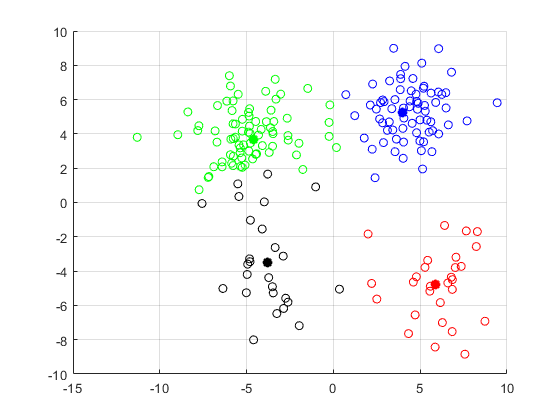
\includegraphics[width=\linewidth]{figs/1-b-meanshift-a.png}
  \caption{$h$ = 5}
  \label{fig:3}
\end{subfigure}

\medskip
\begin{subfigure}{0.25\textwidth}
  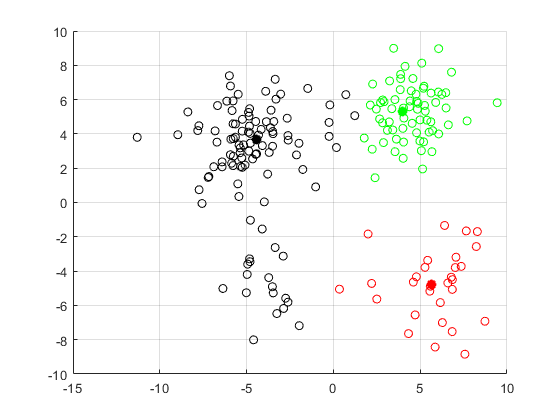
\includegraphics[width=\linewidth]{figs/1-b-meanshift-a-6.png}
  \caption{$h$ = 6}
  \label{fig:4}
\end{subfigure}\hfil % <-- added
\begin{subfigure}{0.25\textwidth}
  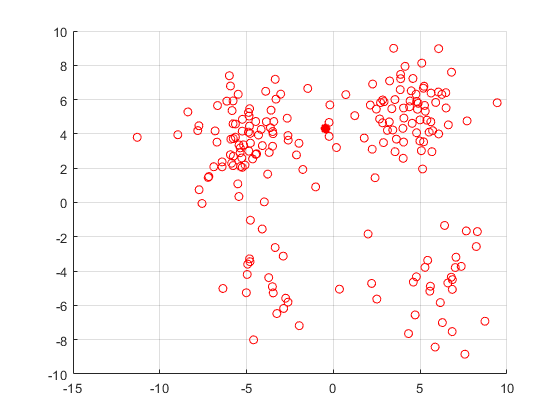
\includegraphics[width=\linewidth]{figs/1-b-meanshift-a-1.png}
  \caption{$h$ = 7}
  \label{fig:5}
\end{subfigure}\hfil % <-- added
\begin{subfigure}{0.25\textwidth}
  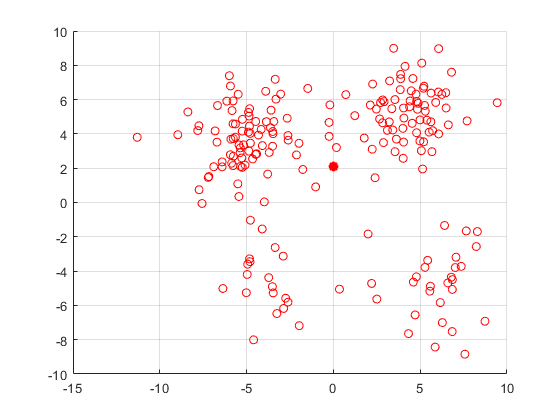
\includegraphics[width=\linewidth]{figs/1-b-meanshift-a-10.png}
  \caption{$h$ = 10}
  \label{fig:6}
\end{subfigure}
\caption{Data\_A}
\label{fig:images}
\end{figure}

\begin{figure}[H]
    \centering % <-- added
\begin{subfigure}{0.25\textwidth}
  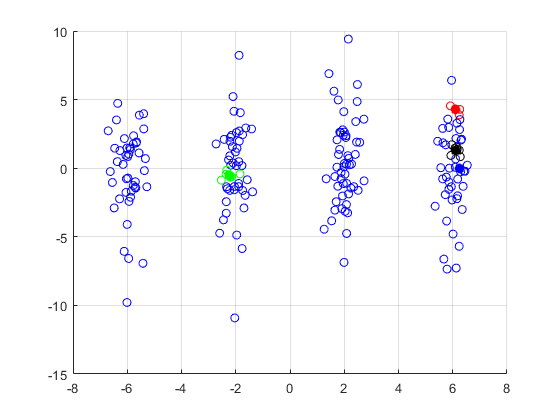
\includegraphics[width=\linewidth]{figs/1-b-meanshift-b-0.png}
  \caption{$h$ = 0.5}
  \label{fig:1}
\end{subfigure}\hfil % <-- added
\begin{subfigure}{0.25\textwidth}
  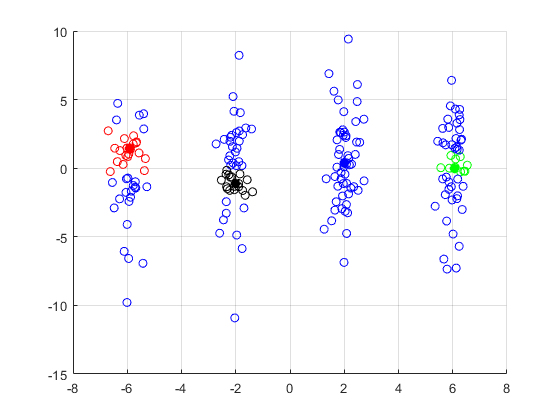
\includegraphics[width=\linewidth]{figs/1-b-meanshift-b-1.png}
  \caption{$h$ = 1}
  \label{fig:2}
\end{subfigure}\hfil % <-- added
\begin{subfigure}{0.25\textwidth}
  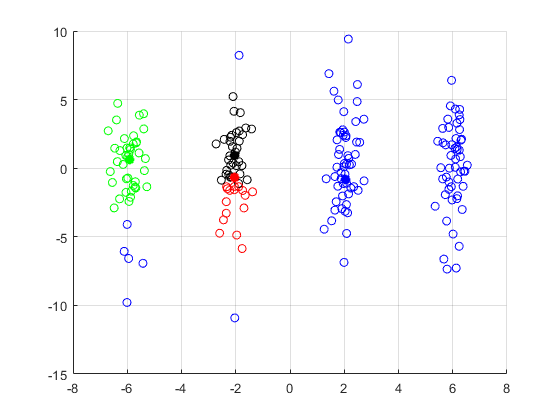
\includegraphics[width=\linewidth]{figs/1-b-meanshift-b-2.png}
  \caption{$h$ = 2}
  \label{fig:3}
\end{subfigure}

\medskip
\begin{subfigure}{0.25\textwidth}
  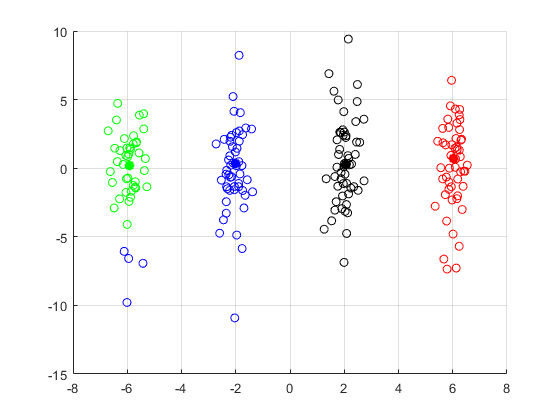
\includegraphics[width=\linewidth]{figs/1-b-meanshift-b.png}
  \caption{$h$ = 3}
  \label{fig:4}
\end{subfigure}\hfil % <-- added
\begin{subfigure}{0.25\textwidth}
  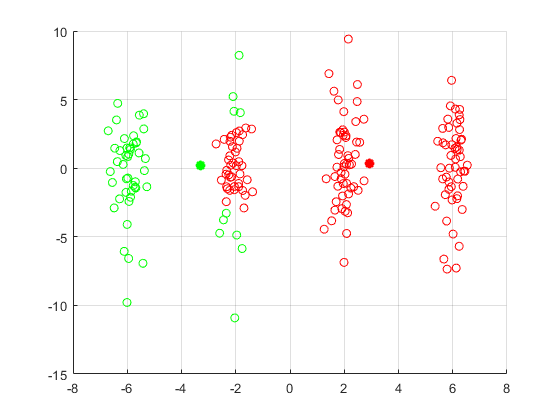
\includegraphics[width=\linewidth]{figs/1-b-meanshift-b-5.png}
  \caption{$h$ = 5}
  \label{fig:5}
\end{subfigure}\hfil % <-- added
\begin{subfigure}{0.25\textwidth}
  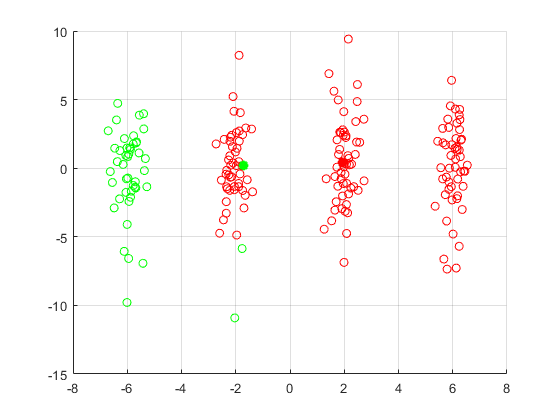
\includegraphics[width=\linewidth]{figs/1-b-meanshift-b-7.png}
  \caption{$h$ = 7}
  \label{fig:6}
\end{subfigure}
\caption{Data\_B}
\label{fig:images}
\end{figure}

\begin{figure}[H]
    \centering % <-- added
\begin{subfigure}{0.25\textwidth}
  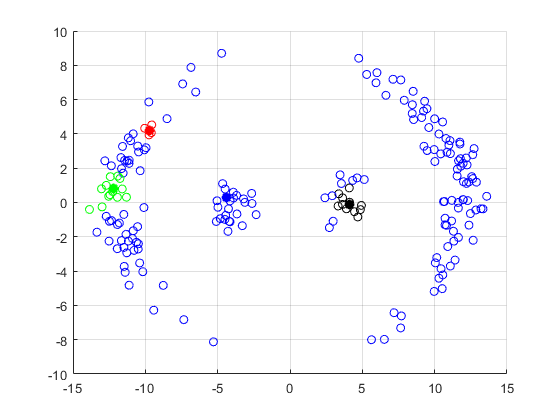
\includegraphics[width=\linewidth]{figs/1-b-meanshift-c-1.png}
  \caption{$h$ = 1}
  \label{fig:1}
\end{subfigure}\hfil % <-- added
\begin{subfigure}{0.25\textwidth}
  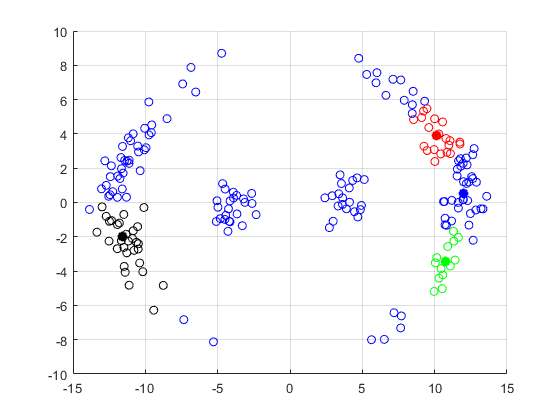
\includegraphics[width=\linewidth]{figs/1-b-meanshift-c-2.png}
  \caption{$h$ = 2}
  \label{fig:2}
\end{subfigure}\hfil % <-- added
\begin{subfigure}{0.25\textwidth}
  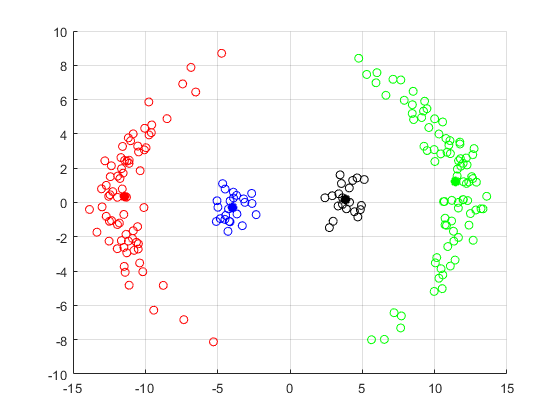
\includegraphics[width=\linewidth]{figs/1-b-meanshift-c-4.png}
  \caption{$h$ = 4}
  \label{fig:3}
\end{subfigure}

\medskip
\begin{subfigure}{0.25\textwidth}
  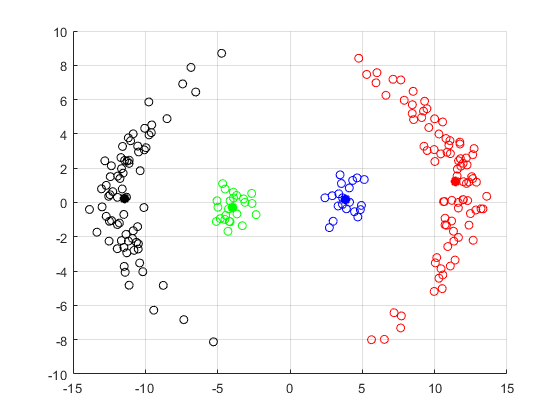
\includegraphics[width=\linewidth]{figs/1-b-meanshift-c.png}
  \caption{$h$ = 5}
  \label{fig:4}
\end{subfigure}\hfil % <-- added
\begin{subfigure}{0.25\textwidth}
  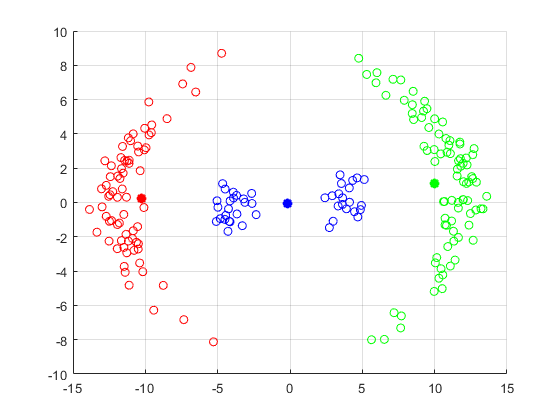
\includegraphics[width=\linewidth]{figs/1-b-meanshift-c-6.png}
  \caption{$h$ = 6}
  \label{fig:5}
\end{subfigure}\hfil % <-- added
\begin{subfigure}{0.25\textwidth}
  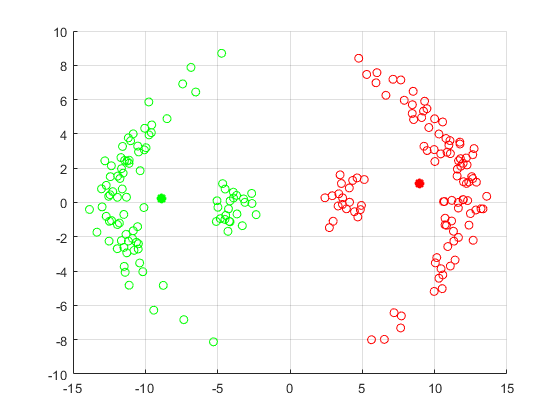
\includegraphics[width=\linewidth]{figs/1-b-meanshift-c-7.png}
  \caption{$h$ = 7}
  \label{fig:6}
\end{subfigure}
\caption{Data\_C }
\label{fig:images}
\end{figure}

\textbf{Conclusion:}\\

From the perspective of the sensitivity of Mean-Shift bandwidth, I test 6 different values on three datasets. In all three datasets, the choice of bandwidth has the general principles. Take Data\_C as an instance. we find that when h = 4 or 5, the clustering results are the best (four distinct results). When the bandwidth is increasing, the cluster number is decreasing into two clusters. Although the cluster number is decreasing, the clustering results are still reflecting the properties of datasets. If the bandwidth is small (e.g. 1,2), it can reflects more details on the data clustering. And it fails to correctly cluster the data sets.

To conclude that, the experiments show that, in order to get better performance on non-parametric clustering, we must know the bandwidth in advance. This is also the limitation of this method.

\section{\fontsize{16}{16}\selectfont Image Segmentation}

\subsection{Segmentation Examples}

\subsubsection{Starfish - Image 12033}

\begin{figure}[H]
	\centering
	\begin{subfigure}[b]{0.475\textwidth}
		\centering
		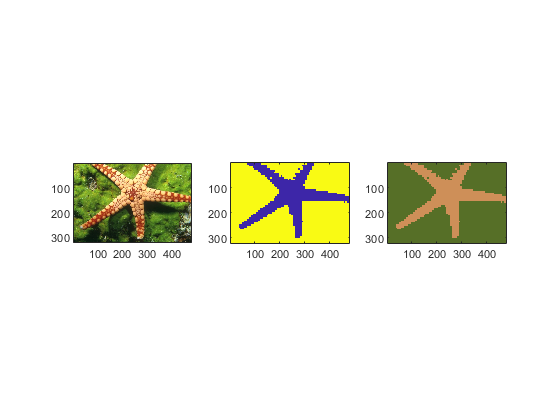
\includegraphics[width=\textwidth]{figs/2-a-kmeans-1}
		\caption[]%
		{{\small K = 2}}    
		\label{fig:mean and std of net14}
	\end{subfigure}
	\hfill
	\begin{subfigure}[b]{0.475\textwidth}  
		\centering 
		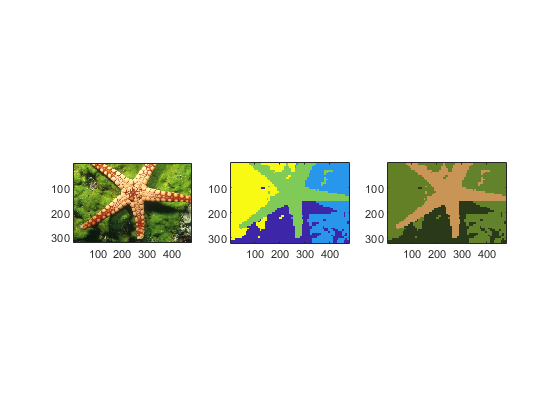
\includegraphics[width=\textwidth]{figs/2-a-kmeans-1-k4}
		\caption[]%
		{{\small  K = 4}}    
		\label{fig:mean and std of net24}
	\end{subfigure}
	\vskip\baselineskip
	\begin{subfigure}[b]{0.475\textwidth}   
		\centering 
		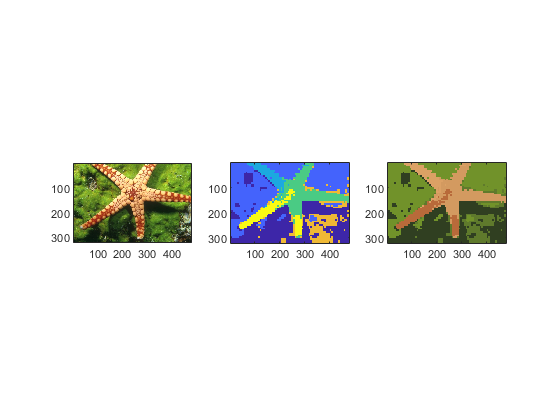
\includegraphics[width=\textwidth]{figs/2-a-kmeans-1-k6}
		\caption[]%
		{{\small  K = 6}}    
		\label{fig:mean and std of net34}
	\end{subfigure}
	\quad
	\begin{subfigure}[b]{0.475\textwidth}   
		\centering 
		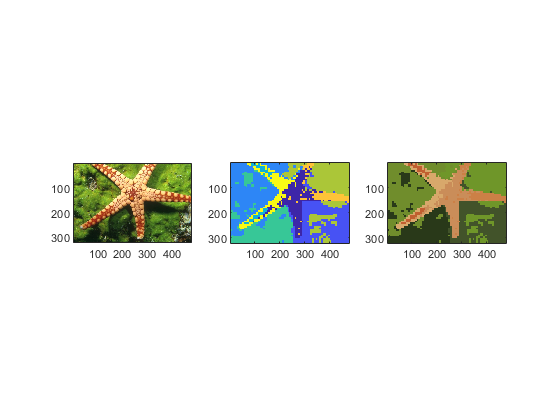
\includegraphics[width=\textwidth]{figs/2-a-kmeans-1-k8}
		\caption[]%
		{{\small  K = 8}}    
		\label{fig:mean and std of net44}
	\end{subfigure}
	\caption[]
	{\small The clustering results using K-means with different k values} 
	\label{fig:mean and std of nets}
\end{figure}

\begin{figure}[H]
	\centering
	\begin{subfigure}[b]{0.475\textwidth}
		\centering
		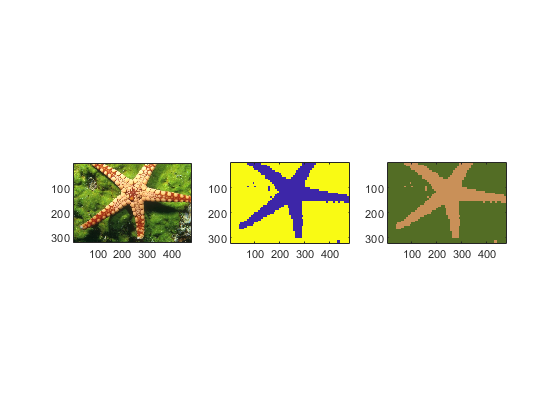
\includegraphics[width=\textwidth]{figs/2-a-em-1}
		\caption[]%
		{{\small K = 2}}    
		\label{fig:mean and std of net14}
	\end{subfigure}
	\hfill
	\begin{subfigure}[b]{0.475\textwidth}  
		\centering 
		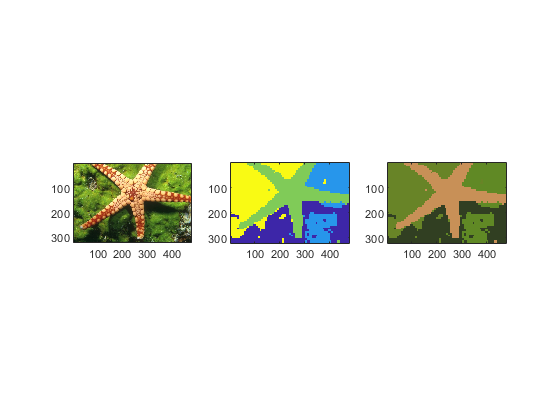
\includegraphics[width=\textwidth]{figs/2-a-em-1-k4}
		\caption[]%
		{{\small  K = 4}}    
		\label{fig:mean and std of net24}
	\end{subfigure}
	\vskip\baselineskip
	\begin{subfigure}[b]{0.475\textwidth}   
		\centering 
		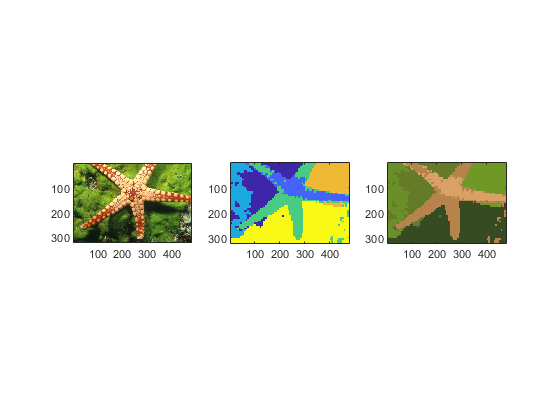
\includegraphics[width=\textwidth]{figs/2-a-em-1-k6}
		\caption[]%
		{{\small  K = 6}}    
		\label{fig:mean and std of net34}
	\end{subfigure}
	\quad
	\begin{subfigure}[b]{0.475\textwidth}   
		\centering 
		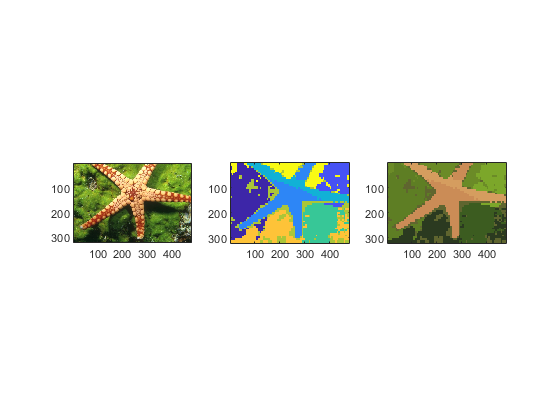
\includegraphics[width=\textwidth]{figs/2-a-em-1-k8}
		\caption[]%
		{{\small  K = 8}}    
		\label{fig:mean and std of net44}
	\end{subfigure}
	\caption[]
	{\small The clustering results using EM-GMM with different k values} 
	\label{fig:mean and std of nets}
\end{figure}

\begin{figure}[H]
	\begin{minipage}{.5\textwidth}
	 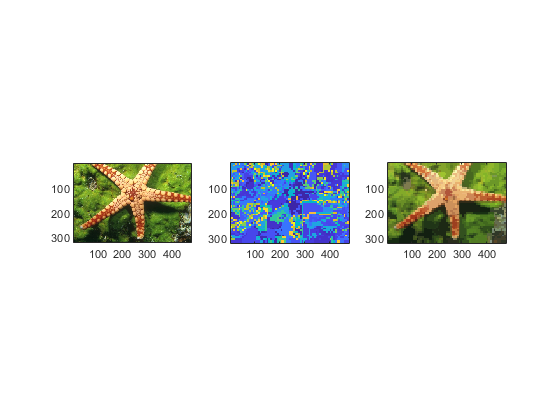
\includegraphics[width=\textwidth,height=\textheight,keepaspectratio]{figs/2-a-ms-1-h4}
	 \caption{\small h = 4}
	\end{minipage}
	\begin{minipage}{.5\textwidth}
	 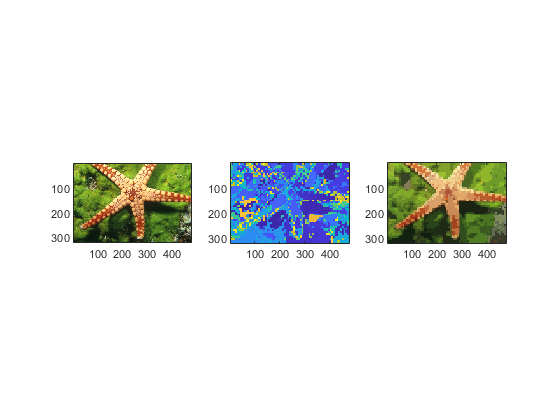
\includegraphics[width=\textwidth,height=\textheight,keepaspectratio]{figs/2-a-ms-1-h5}
	 \caption{\small h = 5}
	\end{minipage}
	\begin{minipage}{.5\textwidth}
		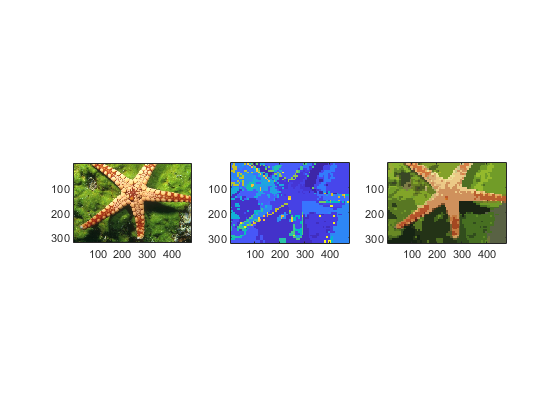
\includegraphics[width=\textwidth,height=\textheight,keepaspectratio]{figs/2-a-ms-1-h7}
		\caption{\small h = 7}
	\end{minipage}
	\caption{The clustering results using Mean-Shift with different bandwidth h values}
  \end{figure}

\subsubsection{Mushroom - Image 208001}

\begin{figure}[H]
	\centering
	\begin{subfigure}[b]{0.475\textwidth}
		\centering
		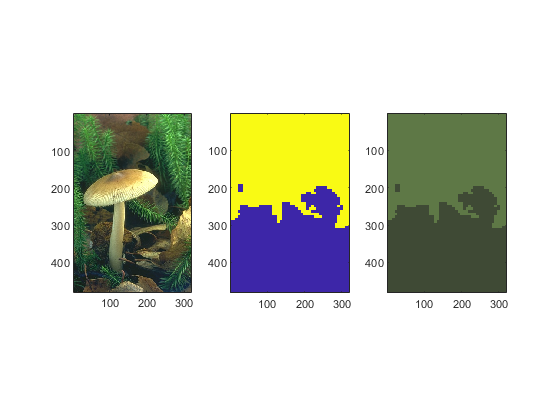
\includegraphics[width=\textwidth]{figs/2-b-kmeans-1-k2}
		\caption[]%
		{{\small K = 2}}    
		\label{fig:mean and std of net14}
	\end{subfigure}
	\hfill
	\begin{subfigure}[b]{0.475\textwidth}  
		\centering 
		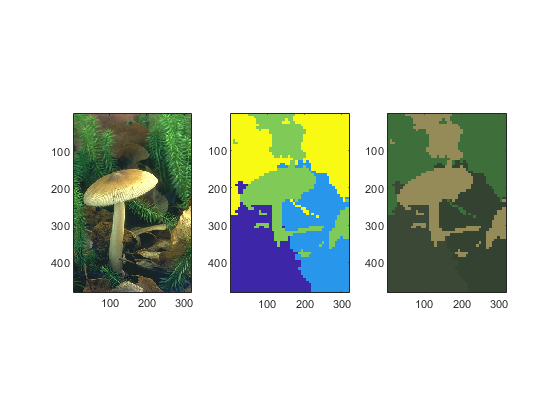
\includegraphics[width=\textwidth]{figs/2-b-kmeans-1-k4}
		\caption[]%
		{{\small  K = 4}}    
		\label{fig:mean and std of net24}
	\end{subfigure}
	\vskip\baselineskip
	\begin{subfigure}[b]{0.475\textwidth}   
		\centering 
		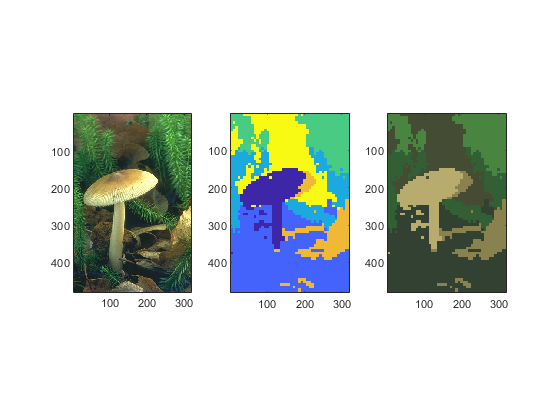
\includegraphics[width=\textwidth]{figs/2-b-kmeans-1-k6}
		\caption[]%
		{{\small  K = 6}}    
		\label{fig:mean and std of net34}
	\end{subfigure}
	\quad
	\begin{subfigure}[b]{0.475\textwidth}   
		\centering 
		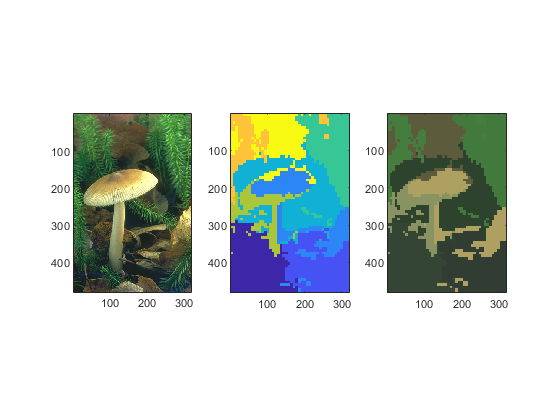
\includegraphics[width=\textwidth]{figs/2-b-kmeans-1-k8}
		\caption[]%
		{{\small  K = 8}}    
		\label{fig:mean and std of net44}
	\end{subfigure}
	\caption[]
	{\small The clustering results using K-means with different k values} 
	\label{fig:mean and std of nets}
\end{figure}


\begin{figure}[H]
	\centering
	\begin{subfigure}[b]{0.475\textwidth}
		\centering
		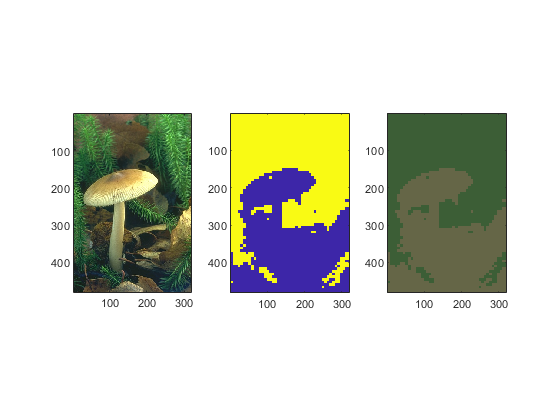
\includegraphics[width=\textwidth]{figs/2-b-em-1-k2}
		\caption[]%
		{{\small K = 2}}    
		\label{fig:mean and std of net14}
	\end{subfigure}
	\hfill
	\begin{subfigure}[b]{0.475\textwidth}  
		\centering 
		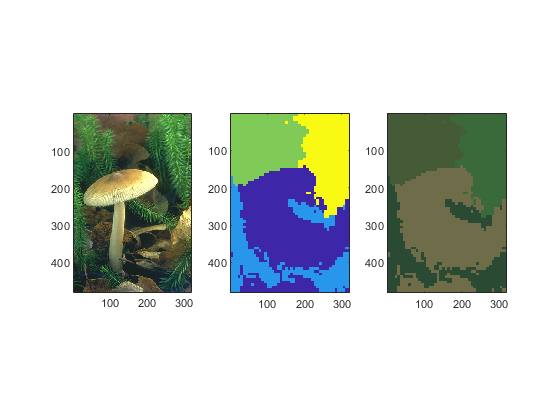
\includegraphics[width=\textwidth]{figs/2-b-em-1-k4}
		\caption[]%
		{{\small  K = 4}}    
		\label{fig:mean and std of net24}
	\end{subfigure}
	\vskip\baselineskip
	\begin{subfigure}[b]{0.475\textwidth}   
		\centering 
		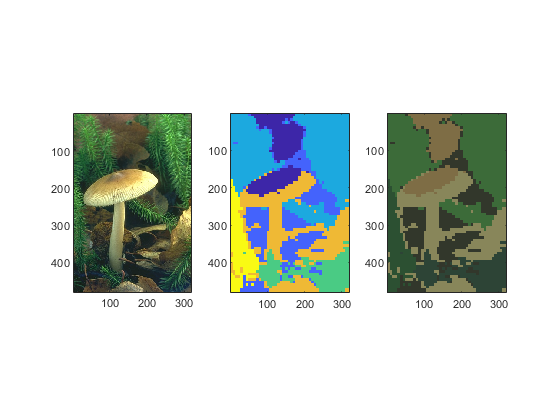
\includegraphics[width=\textwidth]{figs/2-b-em-1-k6}
		\caption[]%
		{{\small  K = 6}}    
		\label{fig:mean and std of net34}
	\end{subfigure}
	\quad
	\begin{subfigure}[b]{0.475\textwidth}   
		\centering 
		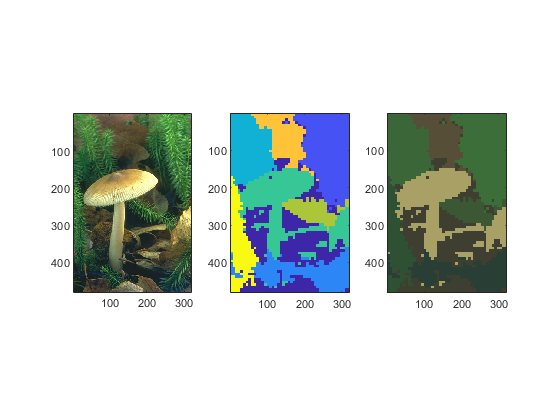
\includegraphics[width=\textwidth]{figs/2-b-em-1-k8}
		\caption[]%
		{{\small  K = 8}}    
		\label{fig:mean and std of net44}
	\end{subfigure}
	\caption[]
	{\small The clustering results using EM-GMM with different k values} 
	\label{fig:mean and std of nets}
\end{figure}

\begin{figure}[H]
	\begin{minipage}{.5\textwidth}
	 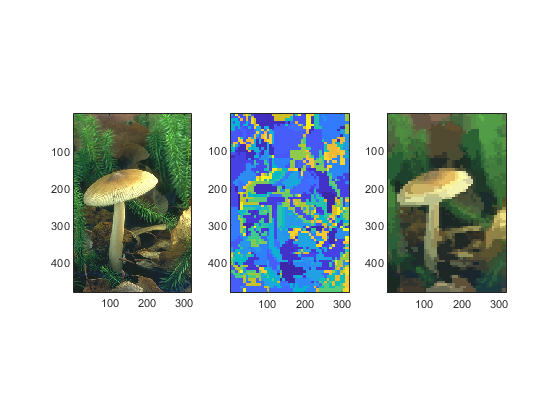
\includegraphics[width=\textwidth,height=\textheight,keepaspectratio]{figs/2-b-ms-1-h4}
	 \caption{\small h = 4}
	\end{minipage}
	\begin{minipage}{.5\textwidth}
	 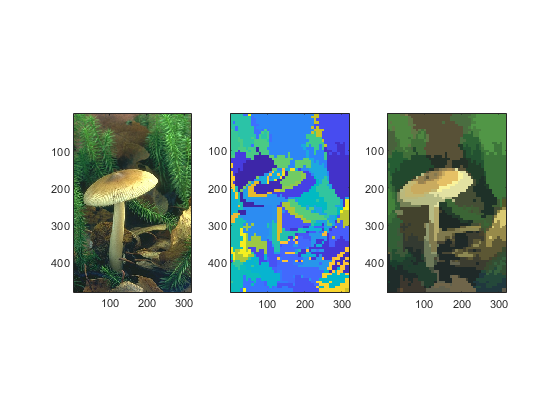
\includegraphics[width=\textwidth,height=\textheight,keepaspectratio]{figs/2-b-ms-1-h6}
	 \caption{\small h = 6}
	\end{minipage}
	\begin{minipage}{.5\textwidth}
		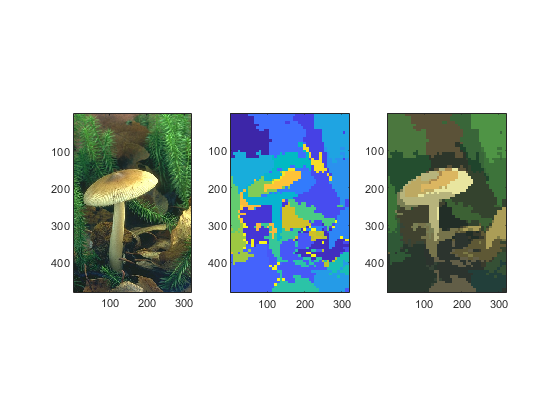
\includegraphics[width=\textwidth,height=\textheight,keepaspectratio]{figs/2-b-ms-1-h8}
		\caption{\small h = 8}
	\end{minipage}
	\caption{The clustering results using Mean-Shift with different bandwidth h values}
  \end{figure}

\textbf{Conclusion:}\\

The picture above shows the evaluation results of three algorithms. What's more, I also adjust the model parameters to make the clustering performance better. Qualitatively, Mean-Shift algorithm has a better performance than EM-GMM and K-means. By adjusting the bandwidth, we can get the best evaluation results using mean-shift algorithm. For Em-GMM and k-means, when we increase the cluster number k, the evaluated results will show more details in both datasets (starfish \& Mushroom). 

When considering the sensitivity of three algorithms, the mean-shift algorithm is the most sensible. For EM-GMM and k-means, even when cluster number k is very small, the segmentation still can represent the shape of original figures. But when bandwidth h is very small or large,the segmentation totally loses the properties of original pictures. 

This example could represent the advantages and limitations of mean-shift algorithm. It doesn't rely assume shape on clusters and has only one parameter choice (bandwidth). Therefore, it is a generic technique for clustering and fit into many different models. The main limitation lies on the selection of window size.

For k-means algorithm, despite of its efficiency and simplicity, it lacks consistency, that means clustering results mainly rely on Initialization sets. When I run the k-means program, the running time tends to be very long if the data set is very large.

For EM-GMM, it provides more information, including latent information, than k-means algorithm. But it needs more computation time and could easily fall into the local maximum. Also it needs us to specify the clustering number K in advance. 

\subsection{Allowing Different Scaling of the Features}

\subsubsection{K-Means}

\begin{figure}[H]
	\centering
	\begin{subfigure}[b]{0.475\textwidth}
		\centering
		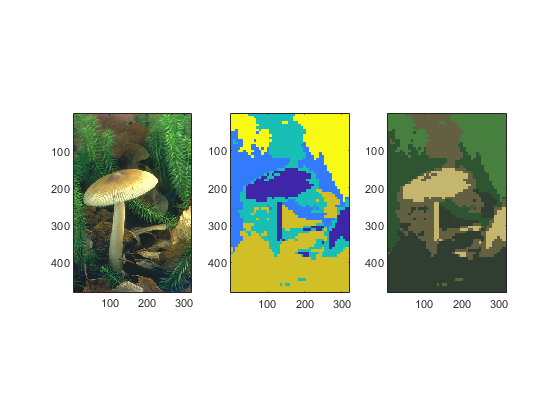
\includegraphics[width=\textwidth]{figs/2-c-ks-5-0-1}
		\caption[]%
		{{\small $\lambda = 0.1$}}    
		\label{fig:mean and std of net14}
	\end{subfigure}
	\hfill
	\begin{subfigure}[b]{0.475\textwidth}  
		\centering 
		\includegraphics[width=\textwidth]{figs/2-c-ks-5-0-5}
		\caption[]%
		{{\small  $\lambda = 0.5$}}    
		\label{fig:mean and std of net24}
	\end{subfigure}
	\vskip\baselineskip
	\begin{subfigure}[b]{0.475\textwidth}   
		\centering 
		\includegraphics[width=\textwidth]{figs/2-c-ks-5-1}
		\caption[]%
		{{\small  $\lambda = 1$}}    
		\label{fig:mean and std of net34}
	\end{subfigure}
	\quad
	\begin{subfigure}[b]{0.475\textwidth}   
		\centering 
		\includegraphics[width=\textwidth]{figs/2-c-ks-5-3}
		\caption[]%
		{{\small  $\lambda = 3$}}    
		\label{fig:mean and std of net44}
	\end{subfigure}
	\caption[]
	{\small The clustering results using K-means with different Scaling values, Clustering number k = 5} 
	\label{fig:mean and std of nets}
\end{figure}

\subsubsection{Mean-Shift}

\begin{figure}[H]
	\centering
	\begin{subfigure}[b]{0.475\textwidth}
		\centering
		\includegraphics[width=\textwidth]{figs/2-c-ms-h6-s0-1}
		\caption[]%
		{{\small $\lambda = 0.1$}}    
		\label{fig:mean and std of net14}
	\end{subfigure}
	\hfill
	\begin{subfigure}[b]{0.475\textwidth}  
		\centering 
		\includegraphics[width=\textwidth]{figs/2-c-ms-h6-s0-5}
		\caption[]%
		{{\small  $\lambda = 0.5$}}    
		\label{fig:mean and std of net24}
	\end{subfigure}
	\vskip\baselineskip
	\begin{subfigure}[b]{0.475\textwidth}   
		\centering 
		\includegraphics[width=\textwidth]{figs/2-c-ms-h6-s1}
		\caption[]%
		{{\small  $\lambda = 1$}}    
		\label{fig:mean and std of net34}
	\end{subfigure}
	\quad
	\begin{subfigure}[b]{0.475\textwidth}   
		\centering 
		\includegraphics[width=\textwidth]{figs/2-c-ms-h6-s3}
		\caption[]%
		{{\small  $\lambda = 3$}}    
		\label{fig:mean and std of net44}
	\end{subfigure}
	\caption[]
	{\small Clustering results using Mean-Shift with different Scaling values, bandwidth h = 6}
	\label{fig:mean and std of nets}
\end{figure}

\textbf{Conclusion}\\

Here, $\lambda$ is defined as the ratio of pixel location and chrominance values. 

For k-means algorithm, if we add more weights on chrominance values than pixel location, the clustering results could get better. It provides more details, which can't be distinguished when $\lambda = 1$. 

For mean-shift algorithm, when we decrease the weights on chrominance values, outputs tend to be more sensitive on pixel locations, which leads to the clustering of nearby data points. When chrominance values raise the weights, it tends to group the data points with the same color (ignoring the location effects). Observing the experiment figures, we can find that the sketch of Mushroom is very clear when $\lambda = 3$, while the sketch tends to be blur when $\lambda = 0.1$.

\bibliographystyle{IEEEtran}
\bibliography{ref.bib}
\end{document}